\section{Evaluation}

\begin{frame}{Evaluation}	
	\begin{itemize}
		\item<+(1)-|alert@+(1)> Classical metrics such as BLUE and METEOR are inadequate in evaluating document-level MT because they evaluate \textbf{average translation quality} at \textbf{sentence-level}. Thus:
		\begin{itemize}
			\item<+(1)-|alert@+(1)> they are unable to capture document-wide phenomena like coherence and cohesion \cite{wong_extending_2012}.
			\item<+(1)-|alert@+(1)> they are not able to measure improvements over discourse phenomena that affect few words but heavily influence fluency and correctness of the translation \cite{muller_large-scale_2018}. E.g. pronomial anaphora.
		\end{itemize}
		\item<+(1)-|alert@+(1)> Evaluation of \textbf{discourse phenomena} can be undertaken with:
			\begin{itemize}
				\item<+(1)-|alert@+(1)> automatic metrics.
				\item<+(1)-|alert@+(1)> test suites.
			\end{itemize}
	\end{itemize}
\end{frame}

\begin{frame}{Evaluation}	
	\begin{figure}
		\centering
		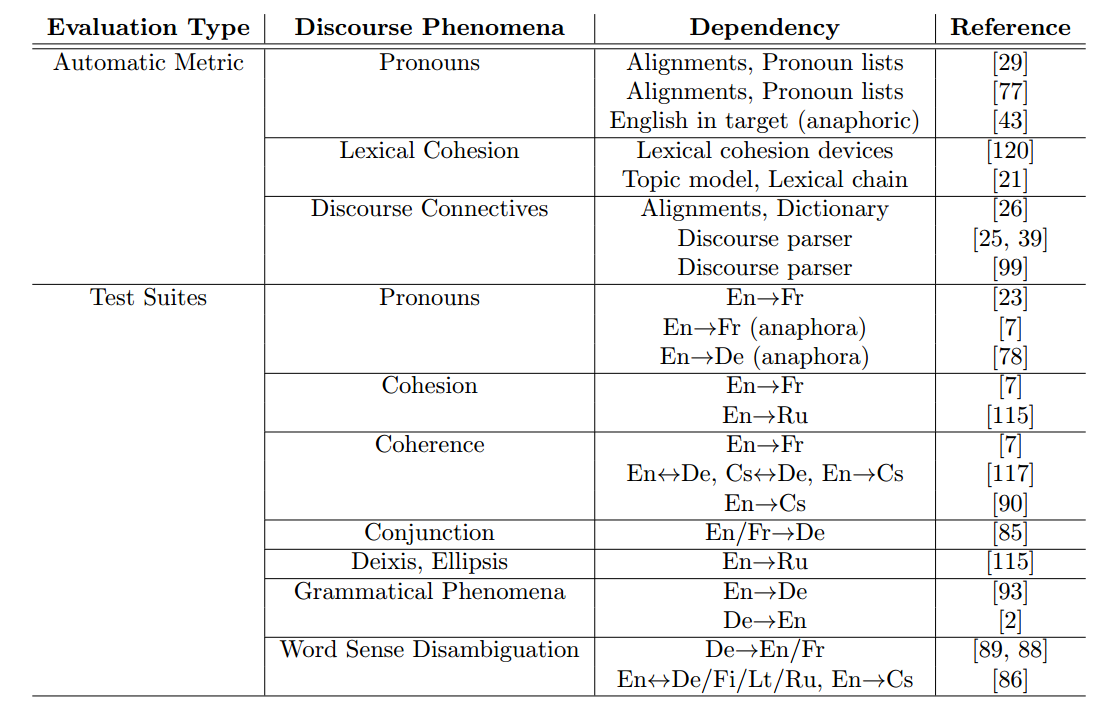
\includegraphics[width=0.7\linewidth]{Images/maruf_2019_discourse_phenomena}
		\caption{Overview of works on discourse phenomena evaluation in MT \cite{maruf_survey_2019}.}
			\label{fig:maruf2019discoursephenomena}
	\end{figure}	
\end{frame}

\begin{frame}{Evaluation}
	The evaluation of discourse-phenomena in document-level MT should:
	\begin{itemize}
		\item<+(1)-|alert@+(1)> Provide inter-sentential context\footnote{in the remainder of this presentation, we refer to inter-sentential context simply as context.}.
		\item<+(1)-|alert@+(1)> Focus on context-dependent cases.
		\begin{itemize}
			\item<+(1)-|alert@+(1)> E.g., pronominal anaphora cases in which the antecedent is in a previous sentence (context-dependent), instead of being in the same sentence (context-independent).
		\end{itemize}
		\item<+(1)-|alert@+(1)> Focus on hard cases.
			\begin{itemize}
				\item<+(1)-|alert@+(1)> E.g., when translating English to French, \textbf{he} is easy whereas \textbf{it} is hard to translate because ambiguous.
			\end{itemize}
	\end{itemize} 
\end{frame}

%%%%%%%%%%%%%%%%%%%%%%%%%%%%%%%%%%%%%%%%%%%%%%%%%%%%%%%%%%%%%%%%%%%%%%%%%

\subsection{Automatic metrics}

\begin{frame}{Automatic metrics}
	\textbf{Accuracy of Pronoun Translation} \cite{miculicich_werlen_validation_2017}:
	\begin{enumerate}
		\item<+(1)-|alert@+(1)> Align source, reference and candidate translation with GIZA++ plus some heuristics.
		\item<+(1)-|alert@+(1)> Compare candidate and reference pronouns taking into account \textbf{equivalent} pronouns and identical pronouns with \textbf{different forms} (target language-specific).
		\begin{itemize}
			\item<+(1)-|alert@+(1)> E.g. \textit{it is difficult} $\rightarrow$ \textit{il/ce/c' est difficile}. 
		\end{itemize}
	\end{enumerate}
	\begin{itemize}
		\item<+(1)-|alert@+(1)> \textit{Compatible languages}: conceived for English to French but it has also been extended to other language pairs. \\
	\end{itemize}
\end{frame}

\begin{frame}{Automatic metrics}	
	\textbf{Pronoun Pair-wise Ranking} \cite{jwalapuram_evaluating_2019}	
	\begin{itemize}
		\item<+(1)-|alert@+(1)> \textit{Rationale}: \textbf{ranking-based evaluation} measures can achieve higher correlations with human judgments, as rankings are simpler to obtain from humans and to train models on.
		\item<+(1)-|alert@+(1)> \textit{Compatible languages}: all target languages on which it is possible to built a training set (parsers needed). all source languages!
		\item<+(1)-|alert@+(1)> \textit{System input}: a pair $R=(C_r, r)$ and $S=(C_s, s)$ of translations to be compared:
		\begin{itemize}
			\item<+(1)-|alert@+(1)> $C_r,C_s$ are the two translations. Each $C$ can comprise one or multiple sentences (context)
			\item<+(1)-|alert@+(1)> $r,s$ are the positions of the pronouns to be compared in the translation $R$ and $S$, respectively.
		\end{itemize} 
	\end{itemize}	
\end{frame}

\begin{frame}{Automatic metrics}	
	\begin{figure}
		\centering
		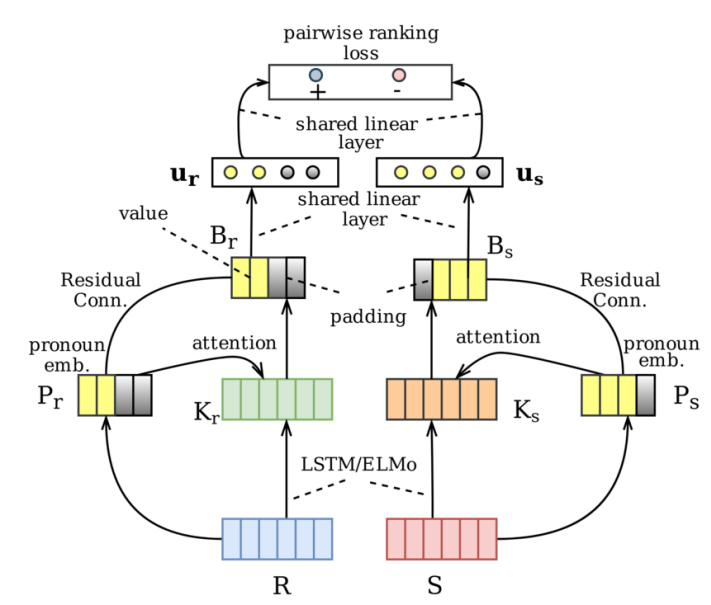
\includegraphics[width=0.55\linewidth]{Images/jwalapuram_2019_pronoun_ranker}
		\caption{Pairwise ranking system by \cite{jwalapuram_evaluating_2019}.}
		\label{fig:jwalapuram2019pronounranker}
	\end{figure}
\end{frame}

\begin{frame}{Automatic metrics}
	\textbf{Lexical Cohesion Devices} \cite{wong_extending_2012}
	\begin{enumerate}
		\item<+(1)-|alert@+(1)> A \textbf{stemming algorithm} \cite{porter_algorithm_1980} is used to identify word stems for each content word  . 
		\begin{itemize}
			\item<+(1)-|alert@+(1)> Words with the same stem are defined and counted as \textbf{Repetitions}.
		\end{itemize}
		\item<+(1)-|alert@+(1)> \textbf{WordNet} \cite{fellbaum_semantic_1998} is used to cluster synonims and superordinates into  semantic groups.
		\begin{itemize}
			\item<+(1)-|alert@+(1)> Words belonging to the same semantic group or close semantic groups (near-synonims) are defined and counted as \textbf{Lexical Cohesion Devices} (LCD).
		\end{itemize}
		\item<+(1)-|alert@+(1)> A \textbf{hybrid metric} can then be defined as weighted average of:		
			\begin{itemize}
				\item<+(1)-|alert@+(1)> a \textbf{classic sentence-level metric}, e.g. BLEU, METEOR, TER.
				\item<+(1)-|alert@+(1)> \textbf{a lexical cohesion metric}, e.g. $Repetitions / content\ words$ or $LCD / content\ words$.
			\end{itemize}
	\end{enumerate}
	\begin{itemize}
		\item<+(1)-|alert@+(1)> \textit{Compatible languages}: all languages with stemmers and WordNets available.
	\end{itemize}
\end{frame}

%%%%%%%%%%%%%%%%%%%%%%%%%%%%%%%%%%%%%%%%%%%%%%%%%%%%%%%%%%%%%%%%%%%%%%%%%

\subsection{Test Suites}

\begin{frame}{Test Suites}\label{fr:test_suites_intro}
	In the literature we can distinguish three kinds of test suites:
	\begin{itemize}
		\item<+(1)-|alert@+(1)> \textbf{Manual test suites} consist in the manual evaluation of a number of test cases (e.g. discourse phenomena) based on a given machine translation task.
		\begin{itemize}
			\item<+(1)-|alert@+(1)> For instance, WMT2019 not only provided ratings for each system output but also some manual evaluation and analysis of the outputs, like the English $\rightarrow$ Czech test suite one on coherence by \cite{rysova_test_2019}.
		\end{itemize}
		\item<+(1)-|alert@+(1)> \textbf{Specialized test sets} are like normal MT test sets but consist of sentence pairs that are more densely populated with specific discourse phenomena. Translations are evaluated on such tests sets by means of average quality metrics like BLEU.
		\begin{itemize}
			\item<+(1)-|alert@+(1)> E.g. \cite{voita_context-aware_2018} build a specialized English $\rightarrow$ Russian test set by retrieving from OpenSubtitles2016 all the sentences containing pronouns that are coreferent to an expression in the previous sentence.
		\end{itemize}
		\item<+(1)-|alert@+(1)> \textbf{Contrastive test suites} consists in blocks of few candidate translations of a given source in which one translation is correct and the others are not. MT systems are assessed on their ability to rank correct translations higher than the incorrect ones.   
	\end{itemize}
\end{frame}

\begin{frame}{Contrastive Test Suites}
	\textbf{Pronomial Anaphora, Lexical Coherence and Cohesion} \cite{bawden_evaluating_2018}
	\begin{itemize}
		\item<+(1)-|alert@+(1)> \textit{Language} English $\rightarrow$ French (OpenSubtitles2016).
		\item<+(1)-|alert@+(1)> One test suite on \textbf{pronomial anaphora} comprised of 50 blocks.
	\end{itemize}
\end{frame}

\begin{frame}{Contrastive Test Suites}
	\begin{figure}
		\centering
		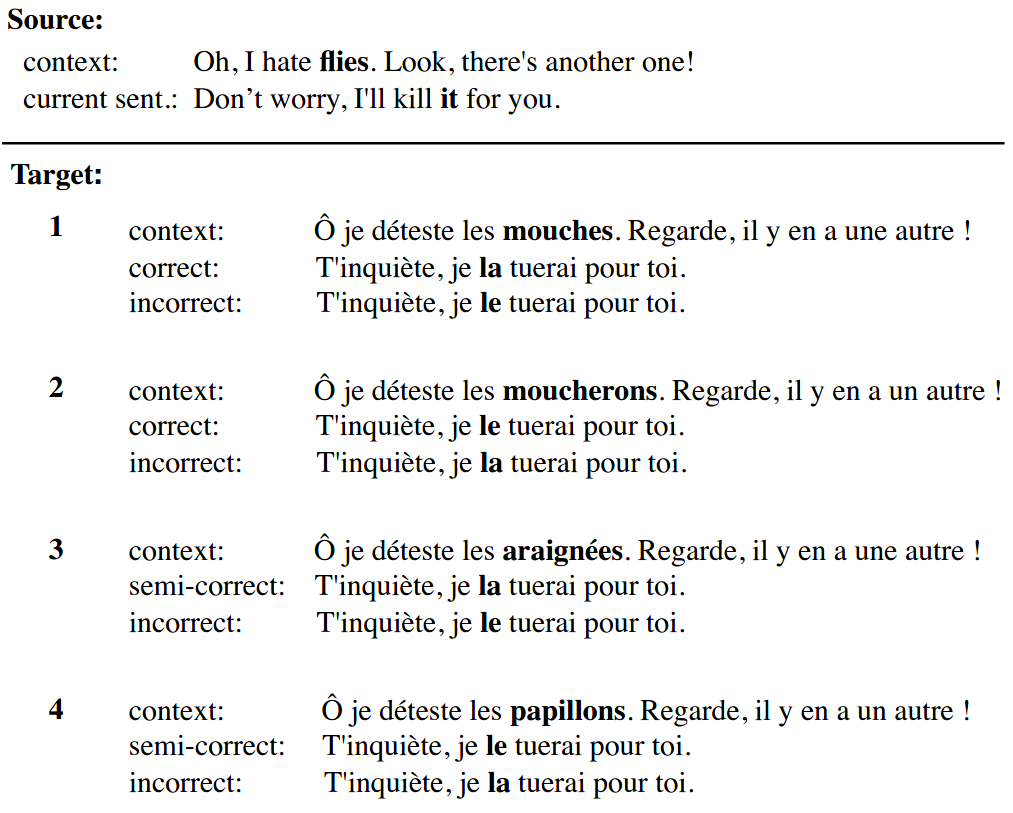
\includegraphics[width=0.59\linewidth]{Images/anaphora_test_suite}
		\caption{Example block of the pronomial anaphora test suite.}
		\label{fig:anaphoratestsuite}
	\end{figure}
% Notes
% different translation of the nominal antecedent for each target element
% two masculine and two feminine
% two semi-correct nominal antecedent translations to test the use of target context by models
\end{frame}

\begin{frame}{Contrastive Test Suites}
	\textbf{Pronomial Anaphora, Lexical Coherence and Cohesion} \cite{bawden_evaluating_2018}
	\begin{itemize}
		\item<+(1)-|alert@+(1)> \textit{Language} English $\rightarrow$ French (OpenSubtitles2016).
		\item<+(1)-|alert@+(1)> One test suite on \textbf{pronomial anaphora} comprised of 50 blocks.
		\item<+(1)-|alert@+(1)> One on \textbf{lexical coherence and cohesion}, comprised of 100 blocks.
	\end{itemize}
\end{frame}


\begin{frame}{Contrastive Test Suites}
	\begin{figure}
		\centering
		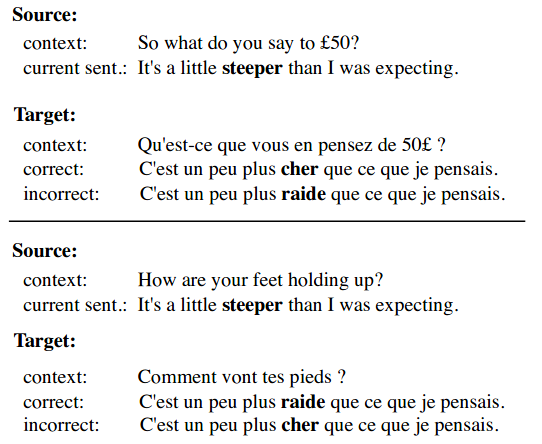
\includegraphics[width=0.57\linewidth]{Images/coherence_test_suite}
		\caption{Example block of the lexical coherence and cohesion test suite.}
		\label{fig:coherencetestsuite}
	\end{figure}
\end{frame}


\begin{frame}{Contrastive Test Suites}
	\textbf{Deixis, Ellipsis, and Lexical Cohesion} \cite{voita_when_2019}
	\begin{itemize}
		\item<+(1)-|alert@+(1)> \textit{Language}: English $\rightarrow$ Russian (OpenSubtitles2018).
		\item<+(1)-|alert@+(1)> \textit{Design method}: manual design preceded by a human analysis on the most common translation errors in the target language pair.
	\end{itemize}
\end{frame}

\begin{frame}{Contrastive Test Suites}
	\textbf{Large Contrastive Test-suite for Pronoun Translation} \cite{muller_large-scale_2018}
	\begin{itemize}
		\item<+(1)-|alert@+(1)> \textit{Rationale}: previous contrastive test suites are not suitable for DLNMT systems because either they \textbf{don't provid context}, or they are \textbf{too small} to provide statistical significance \cite{bawden_evaluating_2018}.
		\item<+(1)-|alert@+(1)> \textit{Language}: English $\rightarrow$ German (OpenSubtitles2016).
		\item<+(1)-|alert@+(1)> \textit{Focus}: \textit{it} $\rightarrow$ \textit{er, sie, es} (hard cases of inter-sentential anaphora).
		\item<+(1)-|alert@+(1)> \textit{Method}:
		\begin{itemize}
			\item<+(1)-|alert@+(1)> \textbf{Align and parse} source-reference pairs with coreference annotators (e.g. CoreNLP for En)
			\item<+(1)-|alert@+(1)> \textbf \textbf{filter} aligned sentences containing aligned pronouns and antecedents.
			\item<+(1)-|alert@+(1)> \textbf{Randomly sample} 4000 instances of each of the three translations of \textit{it} under consideration: \textit{er,sie,es}.
			\item<+(1)-|alert@+(1)> \textbf{Generate two contrastive translations for each} of the 12000 reference translations, by swapping the correct German pronoun with the two incorrect ones.
		\end{itemize} 
	\end{itemize}
\end{frame}

%%%%%%%%%%%%%%%%%%%%%%%%%%%%%%%%%%%%%%%%%%%%%%%%%%%%%%%%%%%%%%%%%%%%%%%%%

\subsection{Remarks and conclusions}

\begin{frame}{Remarks and conclusions}
	\textbf{Automatic Metrics}
	\begin{itemize}
		\item<+(1)-|alert@+(1)>[$+$] They are \textbf{unexpensive} w.r.t. human annotation.
		\item<+(1)-|alert@+(1)>[$+$] they can be easily extended to all languages.
		\item<+(1)-|alert@+(1)>[$-$] They are \textbf{noisy} because they often rely on other imperfect NLP systems. E.g. alignment and coreference systems.
		\item<+(1)-|alert@+(1)>[$-$] They might \textbf{not be enough correlated with human judgment}:
		\begin{itemize}
			\item<+(1)-|alert@+(1)> is the case of APT, for example, which has been shown by \cite{guillou_automatic_2018} not to be suitable to evaluate the translation of pronouns with certain functions.
		\end{itemize}
		\item<+(1)-|alert@+(1)>[$-$] No existing metrics for coherence although it's very relevant for users.
	\end{itemize}
\end{frame}

\begin{frame}{Remarks and conclusions}
	\textbf{Test Suites}
	\begin{itemize}
		\item<+(1)-|alert@+(1)>[$+$] They can evaluate discourse phenomena translations with \textbf{high precision} and, if well designed, \textbf{hig recall}.
		\item<+(1)-|alert@+(1)>[$-$] Excepts for specialized test sets (slide~\ref{fr:test_suites_intro}), test suites have a \textbf{limited scope}: fixed language pair, fixed number of context sentences (past and future). 
		\item<+(1)-|alert@+(1)>[$-$] Contrastive evaluation has \textbf{limited guarantees}: only permits to conclude whether or not the reference translation is more probable than a contrastive variant. It is not guaranteed at all that the MT system will output such reference translation.\footnote{During scoring, the model is also provided with reference translations as target context (easier). Instead, during translation, the model needs to predict the full sequence, thus being subject to beam search failures and error propagation.} 
	\end{itemize}
\end{frame}

\begin{frame}{Remarks and conclusions}
	\textbf{Possible Future Research Directions}
	\begin{itemize}
		\item<+(1)-|alert@+(1)> New automatic metrics strongly tested against human judgment.
			\begin{itemize}
				\item<+(1)-|alert@+(1)> Works on coherence and cohesion are particularly lacking.
			\end{itemize}
		\item<+(1)-|alert@+(1)> Semi-automatic metrics: use a high precision automatic metric and a human to evaluate negative cases.
		\item<+(1)-|alert@+(1)> New test suites for restricted scope.
			\begin{itemize}
				\item<+(1)-|alert@+(1)> Considering other documents other than movie subtitles for building test sets would be interesting for various reasons:
				\begin{itemize}
					\item No multiple speakers, no unavailable context (the video), more phenomena related to future context. 
				\end{itemize}
				 
			\end{itemize}
	\end{itemize}
\end{frame}



		


%\begin{itemize}[noitemsep,topsep=0pt]
%	\item<+(1)-|alert@+(1)><+(1)-|alert@+(1)> BLUE, METEOR, TER for average quality. Not good enough \cite{maruf_survey_2019}.
%	\item<+(1)-|alert@+(1)><+(1)-|alert@+(1)> \cite{bawden_evaluating_2018}: exemplary contrastive test suite, also good model reaching SOTA. Coherence very bad. Need for good models in coherence?
%\end{itemize}